\documentclass[10pt]{article}
\usepackage[margin=1in]{geometry}

\usepackage{amsmath,amssymb,bm,graphicx,booktabs,float,caption}
\captionsetup{font=small,labelfont=bf}
\renewcommand{\thetable}{S\Roman{table}}
\renewcommand{\thefigure}{S\arabic{figure}}
\graphicspath{{../figures/}}
\makeatletter\newcommand{\tabinput}[1]{\@@input #1 }\makeatother
\title{Supplementary Material\\[4pt]\large Lineage and Release Timing in Correlated Errors of Open-Weight Language Models: A Pair-Level Study}
\author{Sudharsan S, S. Kanaga Suba Raja, Shree Harish V, Chin-Shiuh Shieh, Mong-Fong Horng, Lavanya R}
\date{}
\begin{document}
\sloppy
\maketitle
\noindent This supplement holds material moved from the main paper: the per-model precision analysis that motivates the pair-level design (S1), the record of findings withdrawn from the earlier version of this work (S2), and the full table of the post-hoc simulation-gate audit (S3). Every table is generated from the committed outputs by \texttt{scripts/make\_exp04\_tables.py}; the figure by \texttt{scripts/make\_exp04\_figures.py}.

\section*{S1. Why per-model variance decomposition is not enough}\label{sec:precision}

\subsection*{Model and identification}
Let $Y_i$ be a per-model trait (e.g., accuracy), with family $f(i)$ and release quarter $e(i)$:
\begin{equation}
\begin{aligned}
Y_i &= \mu + \alpha_{f(i)} + \beta_{e(i)} + u_i,\\
\alpha &\sim \mathcal{N}(0,\sigma^2_L),\quad \beta \sim \mathcal{N}(0,\sigma^2_E),\quad u \sim \mathcal{N}(0,\sigma^2_U),
\end{aligned}
\label{eq:vc}
\end{equation}
so that $\operatorname{Var}(\mathbf{y}) = \sigma^2_L Z_F Z_F^\top + \sigma^2_E Z_E Z_E^\top + \sigma^2_U I$, with only the intercept as a fixed effect. The variance components are identified when the covariance basis $\{Z_F Z_F^\top, Z_E Z_E^\top, I\}$ is linearly independent. The rank of the fixed-effects dummy design $[\mathbf{1} \mid Z_F \mid Z_E]$, used as the gate in the earlier version of this work, is not the relevant condition for this model: for the sixteen models evaluated there, that design is rank-deficient (rank 14 of 15) while the covariance basis has full rank (3 of 3). Its condition number also depends on the arbitrary choice of reference level (TABLE~\ref{tab:precision}).

\subsection*{Precision}
Identification does not imply precision. For each design we compute the expected restricted-likelihood information $I_{jk} = \tfrac12\operatorname{tr}(P V_j P V_k)$ at four share scenarios (lineage-dominant 0.5/0.2/0.3, era-dominant 0.2/0.5/0.3, balanced, and low-signal 0.1/0.1/0.8), the delta-method standard error of each share, and, as the verdict, the Monte Carlo root-mean-square error (RMSE) of the share estimates under the same REML estimator (500 replicates per scenario). The analytic standard error tracks the Monte Carlo RMSE closely (e.g., 0.289 versus 0.285 for the sixteen-model design), so it can be used before any measurement.

\begin{table}[H]
\caption{\textbf{Precision of family and era variance shares for per-model traits.} FE: fixed-effects dummy design used as a gate in the earlier version; $\kappa$ range is over every choice of reference levels. Covariance-basis rank 3/3 means the variance components are identified. The last column is the worst-case Monte Carlo RMSE of either share across four scenarios (500 replicates each).}
\label{tab:precision}
\centering
\footnotesize
\begin{tabular}{lcccccc}
\toprule
Design & Families & Quarters & FE full rank & $\kappa(X^\top X)$ range & Cov.\ basis & Worst RMSE \\
\midrule
\tabinput{../tables/tab_precision.tex}
\bottomrule
\end{tabular}
\end{table}

No design reaches an RMSE of 0.10 for both shares (TABLE~\ref{tab:precision}): not the sixteen evaluated models (0.30), not the 47-model candidate frame (0.19), and not the 30-model configuration the earlier version described as sufficient (0.19). Removing the single model responsible for the fixed-effects rank deficiency leaves the RMSE unchanged (0.302). The binding constraint is the number of \emph{levels} of each factor: more models per level help only up to a point (with six families and fourteen quarters, 22 models give 0.256 and 47 give 0.189). In staggered designs (Fig.~\ref{fig:scaling}), bringing both shares within $\pm 0.10$ requires on the order of sixty families and fourteen quarters; with eight quarters the era share never falls below about 0.14. Because release quarters are few by construction, a per-model decomposition is a poor instrument for the paper's research questions in populations like those examined here. Within the designs and scenarios examined, this motivates the pair-level design; it does not show that the shares are inestimable under every design, only that the required numbers of families and quarters exceed those available.

\begin{figure}[H]
\centering
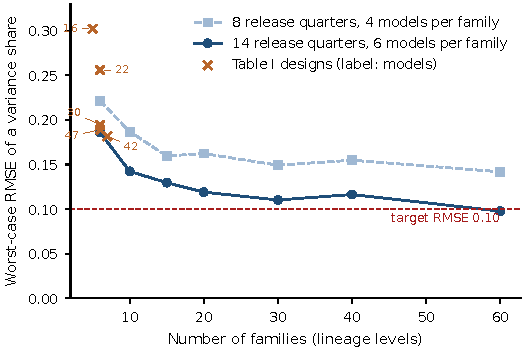
\includegraphics[width=0.7\textwidth]{precision_scaling.pdf}
\caption{\textbf{Precision of per-model variance shares versus the number of families.} Worst-case Monte Carlo RMSE of the family or era share across four scenarios (300 replicates each) for staggered designs with 8 or 14 release quarters, and for the five candidate designs of TABLE~\ref{tab:precision} (crosses, labelled by number of models; 5--7 families). The RMSE is a Monte Carlo root-mean-square error of the estimated share, not the half-width of a confidence interval. The dashed line marks 0.10; only the largest staggered design with 14 quarters (60 families, 360 models) reaches it.}
\label{fig:scaling}
\end{figure}

\section*{S2. Changes from the earlier version}\label{app:v1}
The earlier version of this manuscript (archived in the repository as \texttt{paper/src/archive/}) reported a sixteen-model evaluation and an identifiability gate. TABLE~\ref{tab:v1} lists each finding of that version that is withdrawn or corrected, why, and how it is treated here.

\begin{table}[H]
\caption{\textbf{Findings of the earlier version and their treatment.}}
\label{tab:v1}
\centering
\small
\setlength{\tabcolsep}{2.5pt}
\begin{tabular}{p{0.31\textwidth}p{0.36\textwidth}p{0.27\textwidth}}
\toprule
Earlier claim & Reason & Current treatment \\
\midrule
Variance components ``not identifiable'' (fixed-effects dummy-design gate) & Random-effects model identified (basis rank 3/3); condition number depends on reference level (115--585) & Withdrawn; imprecision quantified (Section~S1) \\
Item-level predictions; Qwen-7B accuracy 0.2294 & Code read only option~A's log-likelihood; 0.2294 is the all-A rate & Withdrawn; code fixed; validation against stored correctness (main paper, Section~IV) \\
30-model design ``passes'' at $\kappa \leq 50$ & Its $\kappa$ is 93 & Corrected \\
Sweep enforced crossing and connectedness & 100 of 105 crossed, 60 connected & Corrected \\
LPM and GLMM both hit the era boundary in 20--60\% of replicates & Only the GLMM; LPM 0--6.7\% & Corrected \\
Nested-design detector: ``zero silent coverage'' & Undefined: no replicate went undetected & Corrected \\
Sixteen-model population as pre-specified & Four planned models not evaluated, no recorded reason; two DeepSeek models imputed & Arm not used for inference \\
\bottomrule
\end{tabular}
\end{table}

\section*{S3. Post-hoc audit of the simulation gate}
The main paper summarizes this audit (Section~III-C and Fig.~3). The table gives every design simulated.

\begin{table}[H]
\caption{\textbf{Post-hoc gate audit} (500 replicates per truth; Wilson 95\% intervals, in percent). Null: largest rejection rate of any term under no effect. Leakage: largest cross-term rejection across $\lambda \in \{0.03, 0.05, 0.10\}$. Power: rejection of the lineage (L) or release-month (E) term. Not pre-specified.}
\label{tab:gateaudit}
\centering
\footnotesize
\resizebox{\textwidth}{!}{\begin{tabular}{lrrcccccc}
\toprule
Sample & Cap & $N$ & Null & Leakage & L, $\lambda{=}0.05$ & E, $\lambda{=}0.05$ & L, $\lambda{=}0.03$ & E, $\lambda{=}0.03$ \\
\midrule
\tabinput{../tables/tab_gateaudit.tex}
\bottomrule
\end{tabular}}
\end{table}

\end{document}
